\documentclass[11pt]{article}

\usepackage[a4paper,margin=1in]{geometry}
\usepackage[utf8]{inputenc}
\usepackage[T1]{fontenc}
\usepackage{lmodern}
\usepackage{microtype}
\usepackage{xcolor}
\usepackage{tikz}
\usetikzlibrary{arrows.meta, positioning, fit, shapes.multipart, shapes.geometric, calc}
\usepackage{listings}
\usepackage{hyperref}
\usepackage{booktabs}
\usepackage{enumitem}
\usepackage{array}
\usepackage{tabularx}
\usepackage{caption}
\usepackage{parskip}

\hypersetup{
    colorlinks=true,
    linkcolor=black,
    citecolor=black,
    urlcolor=blue,
    pdftitle={Mini Transaction Ledger - Technical Explanation Report},
}

\definecolor{codebg}{RGB}{245,245,245}
\definecolor{codekeyword}{RGB}{0,0,140}
\definecolor{codecomment}{RGB}{100,100,100}
\definecolor{codestring}{RGB}{140,0,0}

\lstdefinestyle{code}{
    backgroundcolor=\color{codebg},
    basicstyle=\ttfamily\small,
    keywordstyle=\color{codekeyword}\bfseries,
    commentstyle=\color{codecomment}\itshape,
    stringstyle=\color{codestring},
    breaklines=true,
    frame=single,
    rulecolor=\color{gray!40},
    numbers=left,
    numberstyle=\tiny\color{gray},
    xleftmargin=1.8em,
    tabsize=2,
    showstringspaces=false,
}
\lstset{style=code}

\title{\textbf{Mini Transaction Ledger} \\ \large Technical Explanation Report}
\author{}
\date{\today}

\begin{document}

\maketitle

\tableofcontents
\newpage

\section{Introduction}

Mini Transaction Ledger is a full-stack application for managing financial
accounts and recording transactions against them. A user can create one or
more accounts, post credit and debit entries against those accounts, and
review a running balance history. An administrator role has a separate
view for managing every registered user in the system.

The application is deliberately built around one rule that shapes most of
its backend design: \textbf{a posted transaction is never edited or
deleted}. Corrections are made by posting an offsetting \emph{reversal}
entry, so the transaction log always reflects exactly what happened, in
the order it happened, permanently.

This document explains how the two halves of the application (frontend
and backend) interact, walks through the purpose of the main code
components, describes how a request actually flows through the API, and
explains the Docker setup used to run the whole stack with one command.

\section{Application Architecture}

The system is split into two independently deployable applications that
communicate exclusively over HTTP, plus a shared PostgreSQL database:

\begin{center}
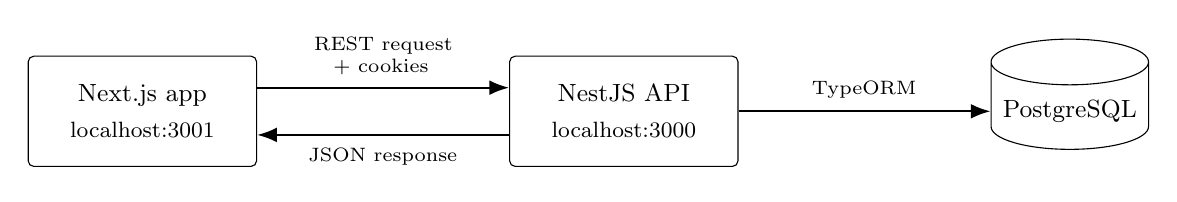
\begin{tikzpicture}[
    node distance=3.2cm,
    box/.style={
        rectangle, draw=black, rounded corners=2pt,
        minimum width=2.9cm, minimum height=1.4cm,
        align=center, font=\small
    },
    db/.style={
        cylinder, draw=black, shape border rotate=90, aspect=0.3,
        minimum width=2cm, minimum height=1.4cm,
        align=center, font=\small
    },
    arrow/.style={-{Latex[length=2.5mm]}, thick},
    lbl/.style={font=\scriptsize, align=center, text width=2.6cm}
]
    \node[box] (frontend) {Next.js app\\[2pt]\footnotesize localhost:3001};
    \node[box, right=of frontend] (backend) {NestJS API\\[2pt]\footnotesize localhost:3000};
    \node[db, right=of backend] (db) {PostgreSQL};

    \draw[arrow] ($(frontend.east)+(0,0.3)$) -- ($(backend.west)+(0,0.3)$)
        node[lbl, midway, above=1pt] {REST request\\+ cookies};
    \draw[arrow] ($(backend.west)+(0,-0.3)$) -- ($(frontend.east)+(0,-0.3)$)
        node[lbl, midway, below=1pt] {JSON response};
    \draw[arrow] (backend) -- (db)
        node[lbl, midway, above=1pt, text width=1.8cm] {TypeORM};
\end{tikzpicture}
\end{center}

The browser (the Next.js client code) talks \textbf{directly} to the
NestJS API using Axios, with \texttt{withCredentials: true} so that
authentication cookies are attached automatically. There is no
server-side proxy, Route Handler, or backend-for-frontend layer sitting
between them --- the frontend is a plain single-page-style client
application, and the only server the browser ever calls is the NestJS
API. Cross-Origin Resource Sharing (CORS) on the backend is restricted to
one configured origin (\texttt{FRONTEND\_URL}) so that only the known
frontend can make authenticated, credentialed requests.

The backend itself is organised into four feature modules, each owning
one database entity, its DTOs (Data Transfer Objects), a service (business
logic and database access), and a controller (HTTP routes and
authorization checks):

\begin{itemize}[nosep]
    \item \textbf{Auth} --- signup, login, token refresh, logout.
    \item \textbf{Users} --- the \texttt{User} entity, roles, admin-only
    user management.
    \item \textbf{Accounts} --- ledger accounts, one-to-many with
    \texttt{User}.
    \item \textbf{Ledger} --- transaction entries, one-to-many with
    \texttt{Account}.
\end{itemize}

The frontend mirrors this with one dedicated API module per backend
resource (\texttt{lib/api/auth.ts}, \texttt{accounts.ts},
\texttt{ledger.ts}, \texttt{users.ts}), and a component tree split the
same way: an authentication page, and a dashboard that renders one of two
completely separate views depending on the logged-in user's role.

\subsection{Database schema}

Three tables model the whole domain: a user owns many accounts, an
account owns many ledger entries, and a ledger entry may optionally point
back at the entry it reverses.

\begin{center}
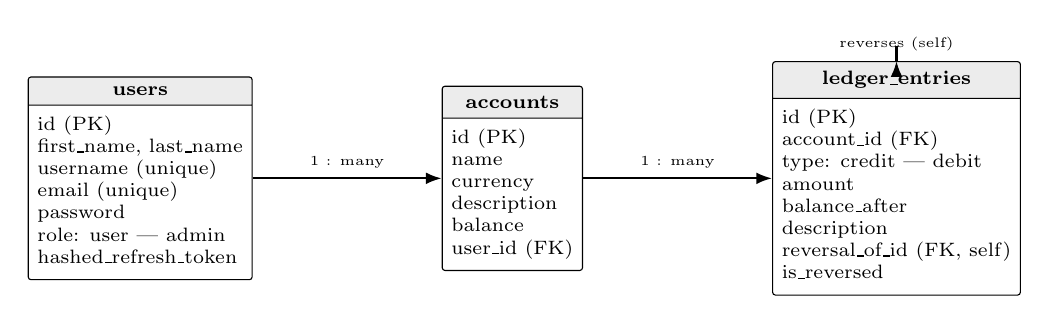
\begin{tikzpicture}[
    node distance=1.6cm and 2.4cm,
    entity/.style={
        rectangle split, rectangle split parts=2,
        rectangle split part align={center,left},
        draw=black, rounded corners=1pt, font=\scriptsize,
        rectangle split part fill={gray!15,white}
    },
    rel/.style={-{Latex[length=2mm]}, thick}
]
    \node[entity] (users) {
        \textbf{users}
        \nodepart{two}
        \begin{tabular}[t]{@{}l@{}}
        id (PK)\\
        first\_name, last\_name\\
        username (unique)\\
        email (unique)\\
        password\\
        role: user | admin\\
        hashed\_refresh\_token
        \end{tabular}
    };

    \node[entity, right=of users] (accounts) {
        \textbf{accounts}
        \nodepart{two}
        \begin{tabular}[t]{@{}l@{}}
        id (PK)\\
        name\\
        currency\\
        description\\
        balance\\
        user\_id (FK)
        \end{tabular}
    };

    \node[entity, right=of accounts] (ledger) {
        \textbf{ledger\_entries}
        \nodepart{two}
        \begin{tabular}[t]{@{}l@{}}
        id (PK)\\
        account\_id (FK)\\
        type: credit | debit\\
        amount\\
        balance\_after\\
        description\\
        reversal\_of\_id (FK, self)\\
        is\_reversed
        \end{tabular}
    };

    \draw[rel] (users) -- (accounts) node[midway, above, font=\tiny] {1 : many};
    \draw[rel] (accounts) -- (ledger) node[midway, above, font=\tiny] {1 : many};
    \draw[rel] (ledger.north) to[out=60,in=120,looseness=6] node[above, font=\tiny] {reverses (self)} (ledger.north);
\end{tikzpicture}
\end{center}

Two foreign-key behaviours are load-bearing for the "never delete ledger
history" rule:

\begin{itemize}[nosep]
    \item \texttt{accounts.user\_id} is \texttt{ON DELETE CASCADE} ---
    deleting a user deletes their accounts, \emph{provided} none of them
    have ledger history.
    \item \texttt{ledger\_entries.account\_id} is \texttt{ON DELETE
    RESTRICT} --- an account (or, by cascade, a user) cannot be deleted
    while it still has ledger entries. The backend catches this specific
    database error and turns it into a clean \texttt{409 Conflict}
    response instead of a raw \texttt{500}.
\end{itemize}

\section{Key Code Components and Their Purpose}

\subsection{Backend (NestJS)}

\begin{description}[style=nextline]
    \item[\texttt{auth/auth.service.ts}] Contains all session logic:
    hashing passwords with bcrypt, issuing an access token (15 minutes)
    and a refresh token (7 days), and verifying a presented refresh token
    against a stored hash before issuing a new pair. The refresh token's
    hash uses SHA-256 with a constant-time comparison rather than bcrypt,
    because bcrypt silently truncates its input to 72 bytes --- since
    every JWT issued to the same user shares an identical header and
    subject-claim prefix, bcrypt would hash them all to the same value,
    making \emph{any} previously issued token match.

    \item[\texttt{auth/strategies/jwt.strategy.ts} \&
    \texttt{refresh-jwt.strategy.ts}] Passport strategies that pull the
    JWT out of an httpOnly cookie (\texttt{access\_token} or
    \texttt{refresh\_token}) rather than an \texttt{Authorization}
    header, and verify its signature and expiry.

    \item[\texttt{auth/guards/jwt-auth.guard.ts},
    \texttt{roles.guard.ts}] Guards run before a controller method. The
    first rejects any request without a valid access token; the second
    reads a \texttt{@Roles(...)} decorator's metadata and rejects the
    request unless the authenticated user's role is in that list.

    \item[\texttt{ledger/ledger.service.ts}] The core business logic for
    posting and reversing transactions. Both operations run inside a
    single database transaction with a pessimistic write lock on the
    account row, so that two concurrent transactions against the same
    account cannot read a stale balance and compute conflicting results.

    \item[\texttt{accounts/accounts.service.ts},
    \texttt{users/users.service.ts}] Both \texttt{remove()} methods catch
    the Postgres foreign-key-restriction error codes
    (\texttt{23503}/\texttt{23001}) and re-throw them as a
    \texttt{ConflictException}, so a doomed delete fails with a clear,
    actionable message instead of an unhandled database exception.

    \item[\texttt{app.module.ts}] Wires every feature module together and
    validates all required environment variables at startup using Joi,
    so a missing configuration value fails fast with a clear error
    instead of an obscure runtime crash later.
\end{description}

\subsection{Frontend (Next.js / React)}

\begin{description}[style=nextline]
    \item[\texttt{lib/api-client.ts}] A thin wrapper around a single
    shared Axios instance. Every backend error response is normalized
    into one \texttt{ApiError} class, and a response interceptor
    transparently retries a failed request once after refreshing the
    session (see Section~\ref{sec:api-internals}).

    \item[\texttt{lib/api/*.ts}] One file per backend resource, each
    exporting a small, named function per endpoint (for example
    \texttt{createEntry}, \texttt{reverseEntry}, \texttt{updateUserRole}).
    Components never call \texttt{fetch}/\texttt{axios} directly ---
    they call these functions, which keeps request shapes and response
    types centralized and typed.

    \item[\texttt{contexts/user-context.tsx}] The application's single
    React Context. It fetches the current session once on mount, exposes
    the logged-in user (or \texttt{null}) and a \texttt{logout} function,
    and is the only piece of global state in the whole frontend.

    \item[\texttt{components/dashboard/*}] The regular-user dashboard:
    an account list and a create-account action on the left, and the
    selected account's balance, transaction table, and
    create/edit/reverse actions on the right. State is deliberately
    ``lifted'' to the nearest shared ancestor
    (\texttt{UserDashboardView}) rather than duplicated in each child.

    \item[\texttt{components/admin/*}] A completely separate dashboard
    rendered only when the session's role is \texttt{admin}: a table of
    every user with role-change and delete actions wired directly to the
    corresponding backend endpoints.
\end{description}

\section{API Endpoint Reference}

Every response is wrapped in the same envelope on success,
\texttt{\{ message, data \}}. In the \textbf{Access} column, \emph{Admin}
means the endpoint requires the \texttt{admin} role via
\texttt{@Roles()}/\texttt{RolesGuard}; \emph{Owner} means it is open to any
authenticated user, but the controller additionally checks that the
requester either owns the resource or is an admin; \emph{User} means any
authenticated user may call it.

\subsection*{Auth --- \texttt{/auth}}

\begin{tabularx}{\textwidth}{@{}llX@{}}
\toprule
Method & Path & Description \\
\midrule
POST & \texttt{/auth/signup} & Register a new user (always created with the \texttt{user} role) \\
POST & \texttt{/auth/login} & Log in with email and password \\
POST & \texttt{/auth/refresh} & Exchange a valid refresh token for a new access/refresh pair \\
POST & \texttt{/auth/logout} & Revoke the current refresh token \\
GET & \texttt{/auth/me} & Get the current session's full user record \\
\bottomrule
\end{tabularx}

\subsection*{Users --- \texttt{/users}}

\begin{tabularx}{\textwidth}{@{}llcX@{}}
\toprule
Method & Path & Access & Description \\
\midrule
POST & \texttt{/users} & Admin & Create a user directly \\
GET & \texttt{/users} & Admin & List all users \\
GET & \texttt{/users/:id} & Owner & Get a single user \\
PATCH & \texttt{/users/:id} & Owner & Update a user (role changes require Admin) \\
DELETE & \texttt{/users/:id} & Admin & Delete a user (fails if their accounts have ledger entries) \\
\bottomrule
\end{tabularx}

\subsection*{Accounts --- \texttt{/accounts}}

\begin{tabularx}{\textwidth}{@{}llcX@{}}
\toprule
Method & Path & Access & Description \\
\midrule
POST & \texttt{/accounts} & User & Create an account for the current user \\
GET & \texttt{/accounts} & User & List accounts (own for \texttt{user}, all for \texttt{admin}) \\
GET & \texttt{/accounts/:id} & Owner & Get a single account \\
PATCH & \texttt{/accounts/:id} & Owner & Update name / description \\
DELETE & \texttt{/accounts/:id} & Owner & Delete an account (fails if it has ledger entries) \\
\bottomrule
\end{tabularx}

\subsection*{Ledger entries --- \texttt{/accounts/:accountId/entries}}

\begin{tabularx}{\textwidth}{@{}llcX@{}}
\toprule
Method & Path & Access & Description \\
\midrule
POST & \texttt{/entries} & Owner & Post a credit or debit entry \\
GET & \texttt{/entries} & Owner & List entries for the account \\
GET & \texttt{/entries/:entryId} & Owner & Get a single entry \\
PATCH & \texttt{/entries/:entryId} & Owner & Update an entry's description only \\
POST & \texttt{/entries/:entryId/reverse} & Owner & Post a reversal of an existing entry \\
\bottomrule
\end{tabularx}

\section{How the API Works Internally}
\label{sec:api-internals}

\subsection{Request lifecycle}

A typical protected request (for example, posting a transaction) passes
through the following stages inside NestJS:

\begin{enumerate}[nosep]
    \item \textbf{Guards} --- \texttt{JwtAuthGuard} verifies the access
    token cookie and attaches the decoded user (\texttt{id}, \texttt{email},
    \texttt{role}) to the request. \texttt{RolesGuard} (where applied)
    checks that role against the endpoint's required roles.
    \item \textbf{Validation pipe} --- the request body is parsed into
    its DTO class and validated with \texttt{class-validator} decorators
    (\texttt{@IsPositive()}, \texttt{@IsEnum()}, etc.); unknown properties
    are stripped, and invalid payloads are rejected with a
    \texttt{400 Bad Request} before any business logic runs.
    \item \textbf{Controller} --- performs any additional ownership check
    (for example, confirming the account being posted to actually belongs
    to the requesting user, or that the user is an admin) and delegates
    to the service.
    \item \textbf{Service} --- contains the actual business logic,
    wrapped in a database transaction where atomicity matters (posting or
    reversing a ledger entry).
    \item \textbf{Serialization} --- the response entity passes through a
    global \texttt{ClassSerializerInterceptor}, which strips fields
    marked \texttt{@Exclude()} (the password hash, the refresh token
    hash) before the JSON reaches the client.
\end{enumerate}

Every successful response is wrapped in the same shape,
\texttt{\{ message, data \}}, which the frontend's \texttt{ApiError}
handling and per-endpoint functions rely on consistently.

\subsection{Authentication and the refresh cycle}

Two JSON Web Tokens are used, both delivered as \texttt{httpOnly} cookies
so they are never reachable from client-side JavaScript:

\begin{itemize}[nosep]
    \item An \textbf{access token} (15 minutes), carrying the user's id,
    email, and role, required on every protected request.
    \item A \textbf{refresh token} (7 days), used only to obtain a new
    access token. Its hash is stored on the user record so that a stolen
    or replayed refresh token can be detected: if a presented token does
    not match the stored hash, the stored hash is cleared, immediately
    revoking that session.
\end{itemize}

Because the access token's role claim is only as fresh as the moment it
was issued, a role change made through the admin dashboard does not take
effect for that user's already-open session until their token is
refreshed. Rather than requiring a manual logout, the frontend handles
this automatically:

\begin{lstlisting}[caption={Automatic refresh-and-retry, from \texttt{lib/api-client.ts}}]
httpClient.interceptors.response.use(
  (response) => response,
  async (error) => {
    const config = error.config;
    const status = error.response?.status;

    const canRetry =
      config &&
      !config._retriedAfterRefresh &&
      (status === 401 || status === 403) &&
      !AUTH_RETRY_EXEMPT_PATHS.some((p) => config.url?.startsWith(p));

    if (canRetry) {
      config._retriedAfterRefresh = true;
      try {
        await refreshSession(); // POST /auth/refresh
        return await httpClient.request(config);
      } catch {
        // refresh failed too; fall through to the original error
      }
    }

    return Promise.reject(error);
  },
);
\end{lstlisting}

Any \texttt{401}/\texttt{403} response (other than from the auth
endpoints themselves) triggers exactly one call to
\texttt{POST /auth/refresh}, which re-reads the user from the database
and re-issues both tokens with the current role; the original request is
then retried once with the fresh cookies already in place. Concurrent
failures share a single in-flight refresh call rather than each starting
their own.

\subsection{The ledger's append-only model}

Posting a transaction never simply increments or decrements a balance in
isolation --- it is always done inside one database transaction that:

\begin{enumerate}[nosep]
    \item Acquires a pessimistic write lock on the account row.
    \item Computes the new balance from the currently locked value.
    \item Inserts the new \texttt{ledger\_entries} row, stamped with that
    resulting \texttt{balance\_after}.
    \item Writes the new balance back onto the account row.
\end{enumerate}

\begin{lstlisting}[caption={Simplified core of \texttt{LedgerService.createEntry}}]
return this.dataSource.transaction(async (manager) => {
  const account = await manager.findOne(Account, {
    where: { id: accountId },
    lock: { mode: 'pessimistic_write' },
  });

  const balanceAfter = this.applyEntry(account.balance, dto.type, dto.amount);

  const entry = manager.create(LedgerEntry, {
    accountId, type: dto.type, amount: dto.amount,
    balanceAfter, description: dto.description ?? null,
  });

  account.balance = balanceAfter;
  await manager.save(account);
  return manager.save(entry);
});
\end{lstlisting}

Because ledger entries model real financial events, they are never
updated or deleted after posting --- only the \texttt{description} field
can be edited afterwards, via a separate endpoint. A mistake is corrected
by \emph{reversing} an entry: a new entry of the opposite type, for the
same amount, is posted and linked back to the original via
\texttt{reversal\_of\_id}, while the original is flagged
\texttt{is\_reversed = true}. This keeps every entry that was ever posted
permanently visible, mistakes included, which is the entire point of an
audit-grade ledger.

\section{Docker Setup Explanation}

The whole stack --- database, API, and frontend --- is brought up with a
single \texttt{docker compose up --build} from the repository root. The
root \texttt{docker-compose.yml} defines three services:

\begin{description}[style=nextline]
    \item[\texttt{postgres}] Uses the official \texttt{postgres:16-alpine}
    image directly (no custom Dockerfile needed). A named volume
    (\texttt{postgres\_data}) persists data across container restarts,
    and a \texttt{healthcheck} runs \texttt{pg\_isready} so that the
    backend does not attempt to connect before the database is actually
    ready to accept connections.

    \item[\texttt{backend}] Built from \texttt{backend/Dockerfile}, a
    three-stage build: a \texttt{deps} stage installs dependencies with
    pnpm (including the \texttt{python3}/\texttt{make}/\texttt{g++}
    toolchain that \texttt{bcrypt}'s native module needs to compile on
    Alpine Linux), a \texttt{build} stage runs \texttt{nest build} to
    produce \texttt{dist/}, and a final \texttt{runtime} stage copies
    only the compiled output and \texttt{node\_modules} into a fresh
    image and runs \texttt{node dist/main}. Configuration (database
    credentials, JWT secrets, the frontend's origin for CORS) is injected
    entirely through environment variables at container start, sourced
    from the root \texttt{.env} file via Compose's variable
    substitution --- \texttt{DB\_HOST} is overridden to the service name
    \texttt{postgres} so the backend reaches the database over the
    Compose-managed Docker network rather than \texttt{localhost}.

    \item[\texttt{frontend}] Built from \texttt{frontend/Dockerfile},
    following the same three-stage pattern, but using Next.js's
    \texttt{output: "standalone"} build mode, which produces a minimal,
    self-contained server bundle. Because
    \texttt{NEXT\_PUBLIC\_BACKEND\_URL} is inlined into the client
    JavaScript bundle at build time (not read at runtime), it is passed
    in as a Docker build \texttt{ARG} rather than a plain environment
    variable, and is set to \texttt{http://localhost:3000} --- the
    address the \emph{browser}, not the container, needs to reach the
    API on the published host port.
\end{description}

Only the database port (5432), the API port (3000), and the frontend port
(3001) are published to the host, matching exactly how the same three
services are addressed when run locally without Docker. A single root
\texttt{.env.example} (copied to \texttt{.env} before the first run)
supplies every value the compose file's variable substitution needs, so
a fresh clone requires no manual configuration beyond that one copy.

\section{Conclusion}

The application separates concerns cleanly along two axes: a frontend/
backend split communicating over a typed, credentialed REST API, and a
backend split into four self-contained feature modules. Authentication
uses short-lived, role-bearing access tokens backed by a longer-lived,
rotation-aware refresh token, with the frontend transparently keeping
itself in sync when a role changes mid-session. The ledger itself is
modelled as an append-only log with a self-referencing reversal pattern
and database-level delete protection, so that the system's core
guarantee --- transaction history is permanent --- is enforced at the
database, not just trusted to application code. The entire stack,
including the database, is reproducible with a single Docker Compose
command.

\end{document}
